\documentclass[../document.tex]{subfiles}
\begin{document}
\chapter{Methodology}
We developed a framework to learn traversability directly on ground patches for any robot using purely simulated data. The core idea, originally proposed by Chavez-Garcia et al. \cite{omar2018traversability}, is simple yet elegant, a robot is let travel into a simulator on different synthetic terrains, while storing its interactions to later crop a region of ground, a patch, around each traveled position and directly train a neural network on them to predict traversability. Figure \ref{fig : pipeline} shows the framework's steps.

\begin{figure}[H]
    \centering
        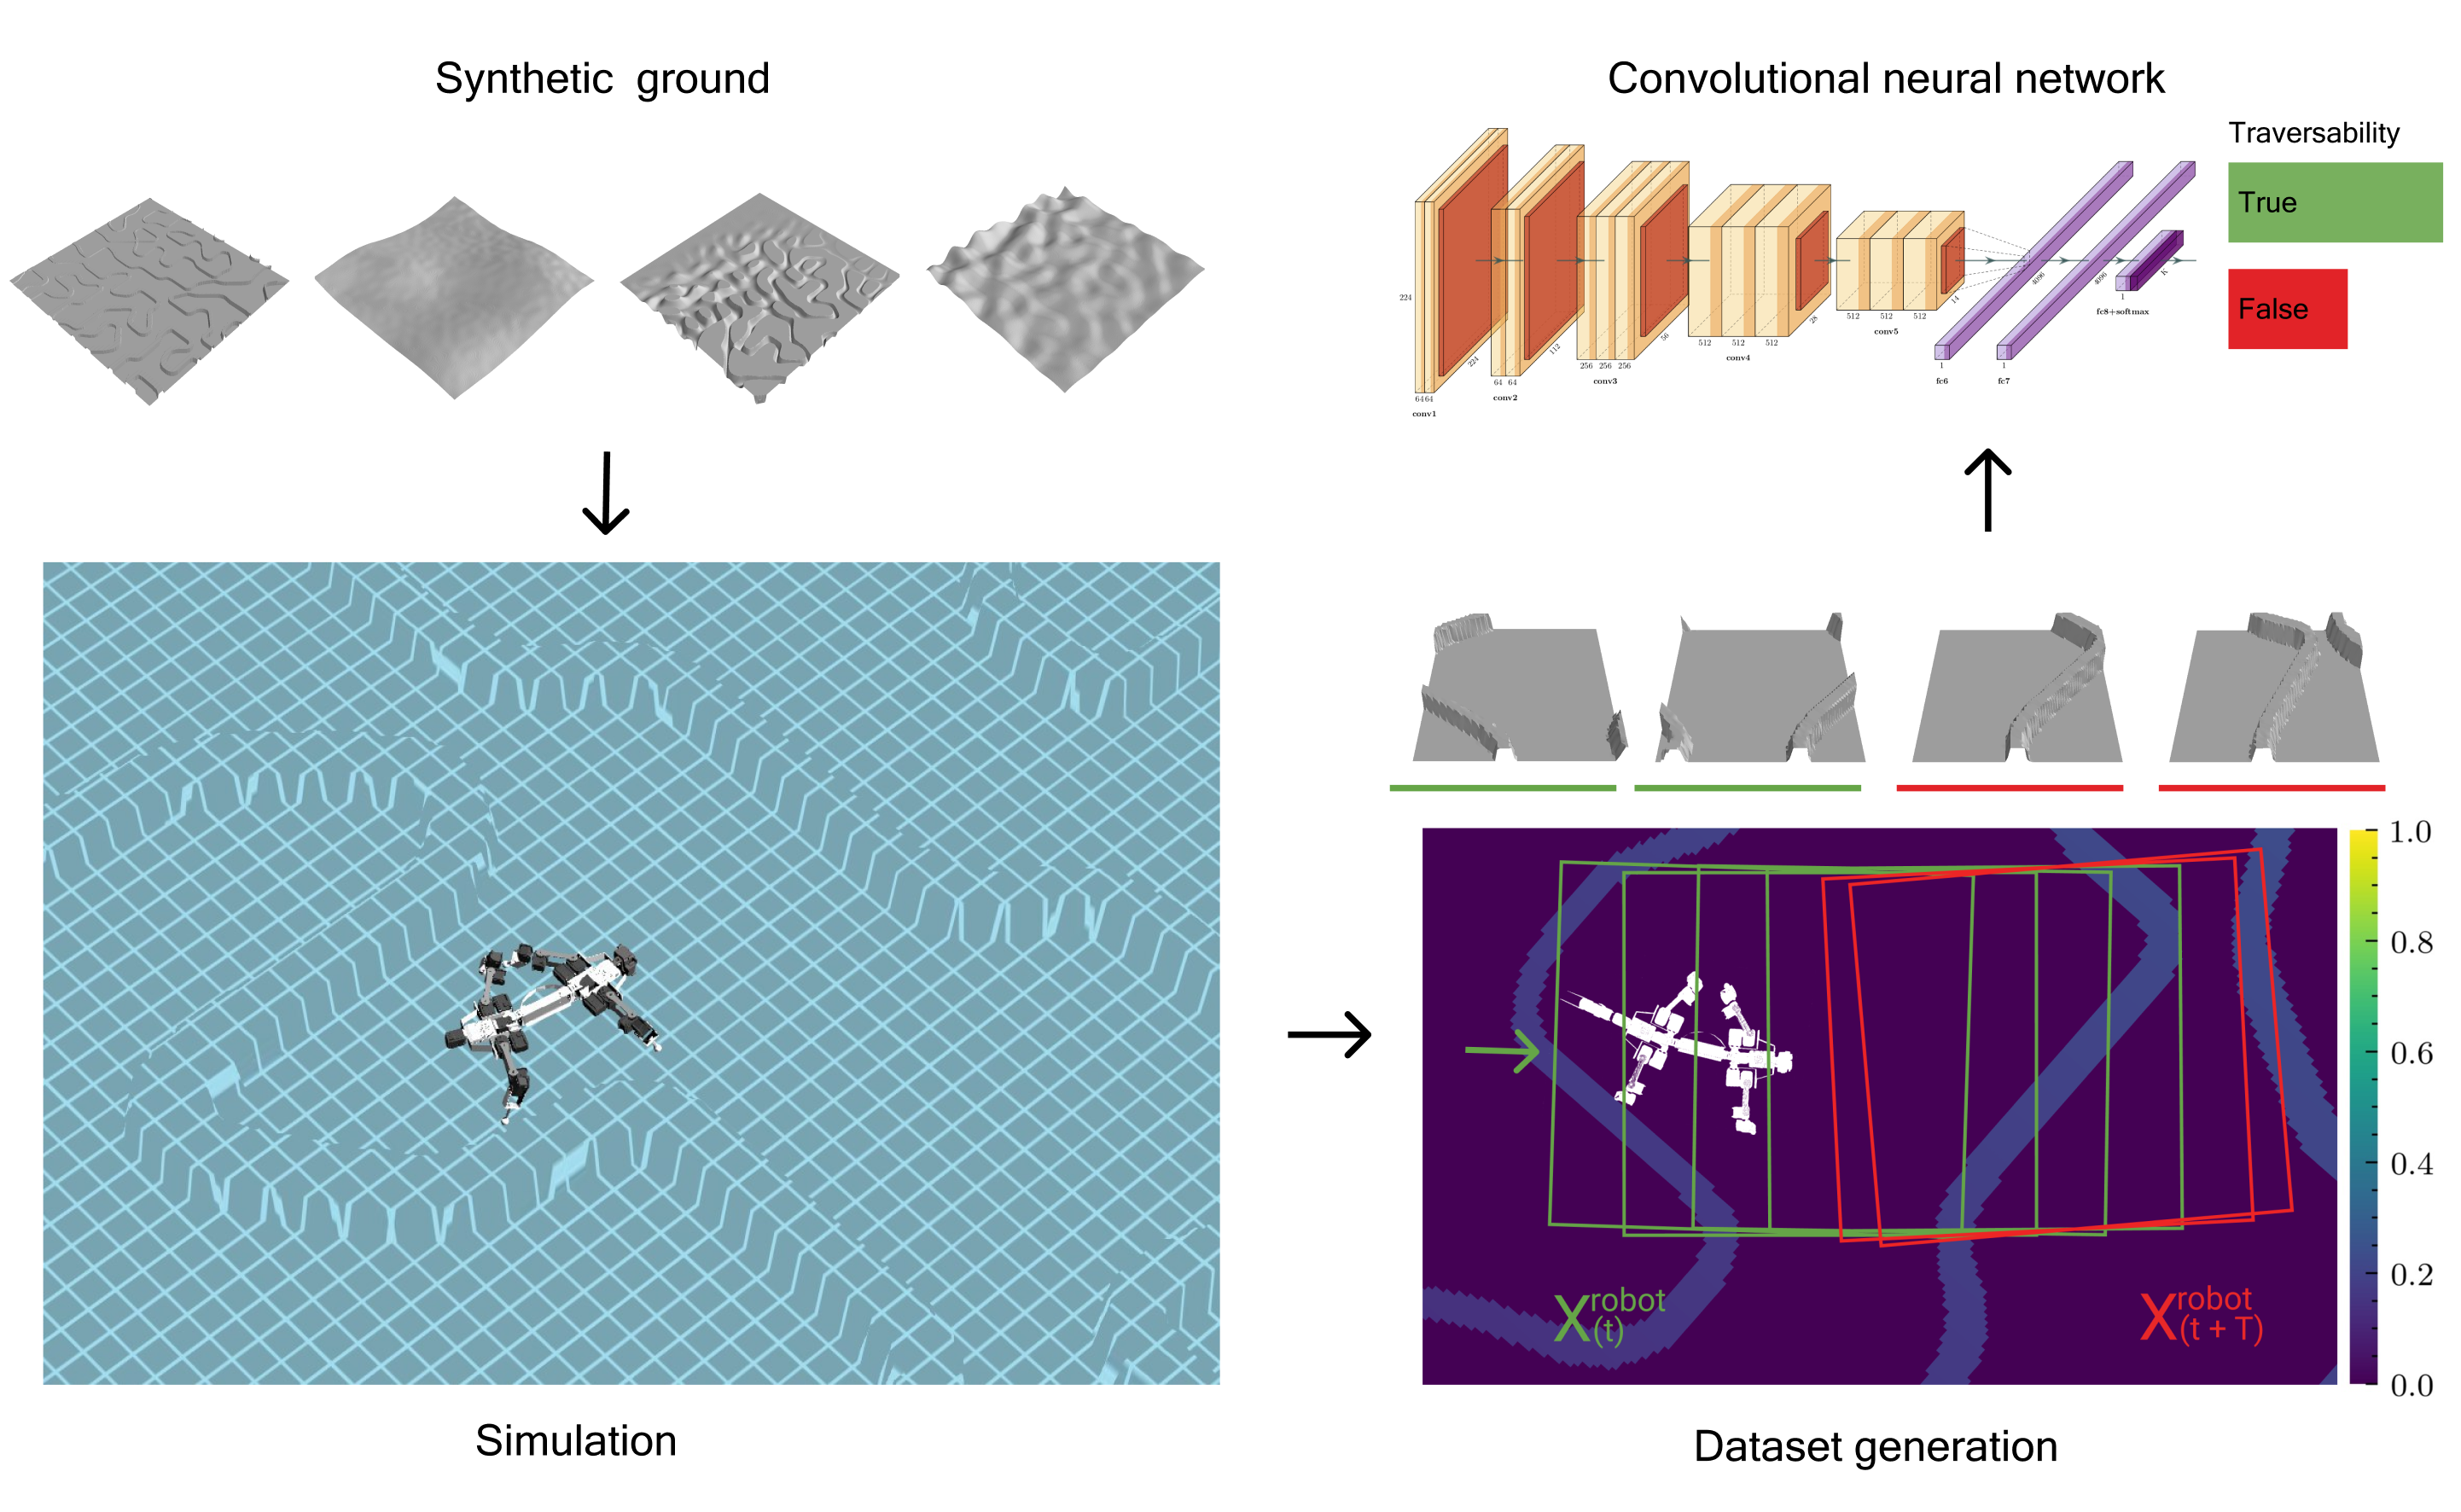
\includegraphics[width=\textwidth]{../img/method.png}
    \caption{The framework's main building block in counter-clockwise order. First, we generated meaningful synthetic grounds, then we let the robot spawn and walk on them in a simulated environment while storing its interactions. Later, we crop a region of ground, a patch, for each simulation trajectory around the robot according to its locomotion. We labeled those images using a defined threshold and fit a deep convolutional neural network to predict traversability. }
    \label{fig : pipeline}
    \end{figure}
Collecting data through simulation has several main advantages such as variety, cost, and speed. With simulations, we can easily increase the number of data samples at any time by simply incorporate more maps. Contrarily, a real robot requires to first identify the suitable ground and then physically transport the machine there and finally let it walk on it.
Furthermore, we are not limited by real constraint and we can design the ground to maximize the variety of robot interactions. We can artificial design maps to include any kind of situations and challenges.
Clearly, this also reduces the time required to collect the robot's interactions with the terrain. The time could be further minimized by running different simulations in parallel bypassing the demand for more physical hardware.
To create a quality dataset, we must generate a series of various surfaces and ensure their diversity. Intuitively, those maps should be small enough to allow fast exploration but big enough to include several features. With modern ground generation techniques, it is fairly straightforward to generate a rich array of terrains with different characteristics such us bumps, ramps, slopes in different levels and sizes. There are several methods to represent terrain, we utilize heightmap where the height component of the ground is stored as pixels in a gray image. Practically, the brightness describes the height. The following figure shows a small collection of synthetic terrains with different features.
\begin{figure}[H]
    \centering
    \begin{subfigure}[b]{0.24\textwidth}
        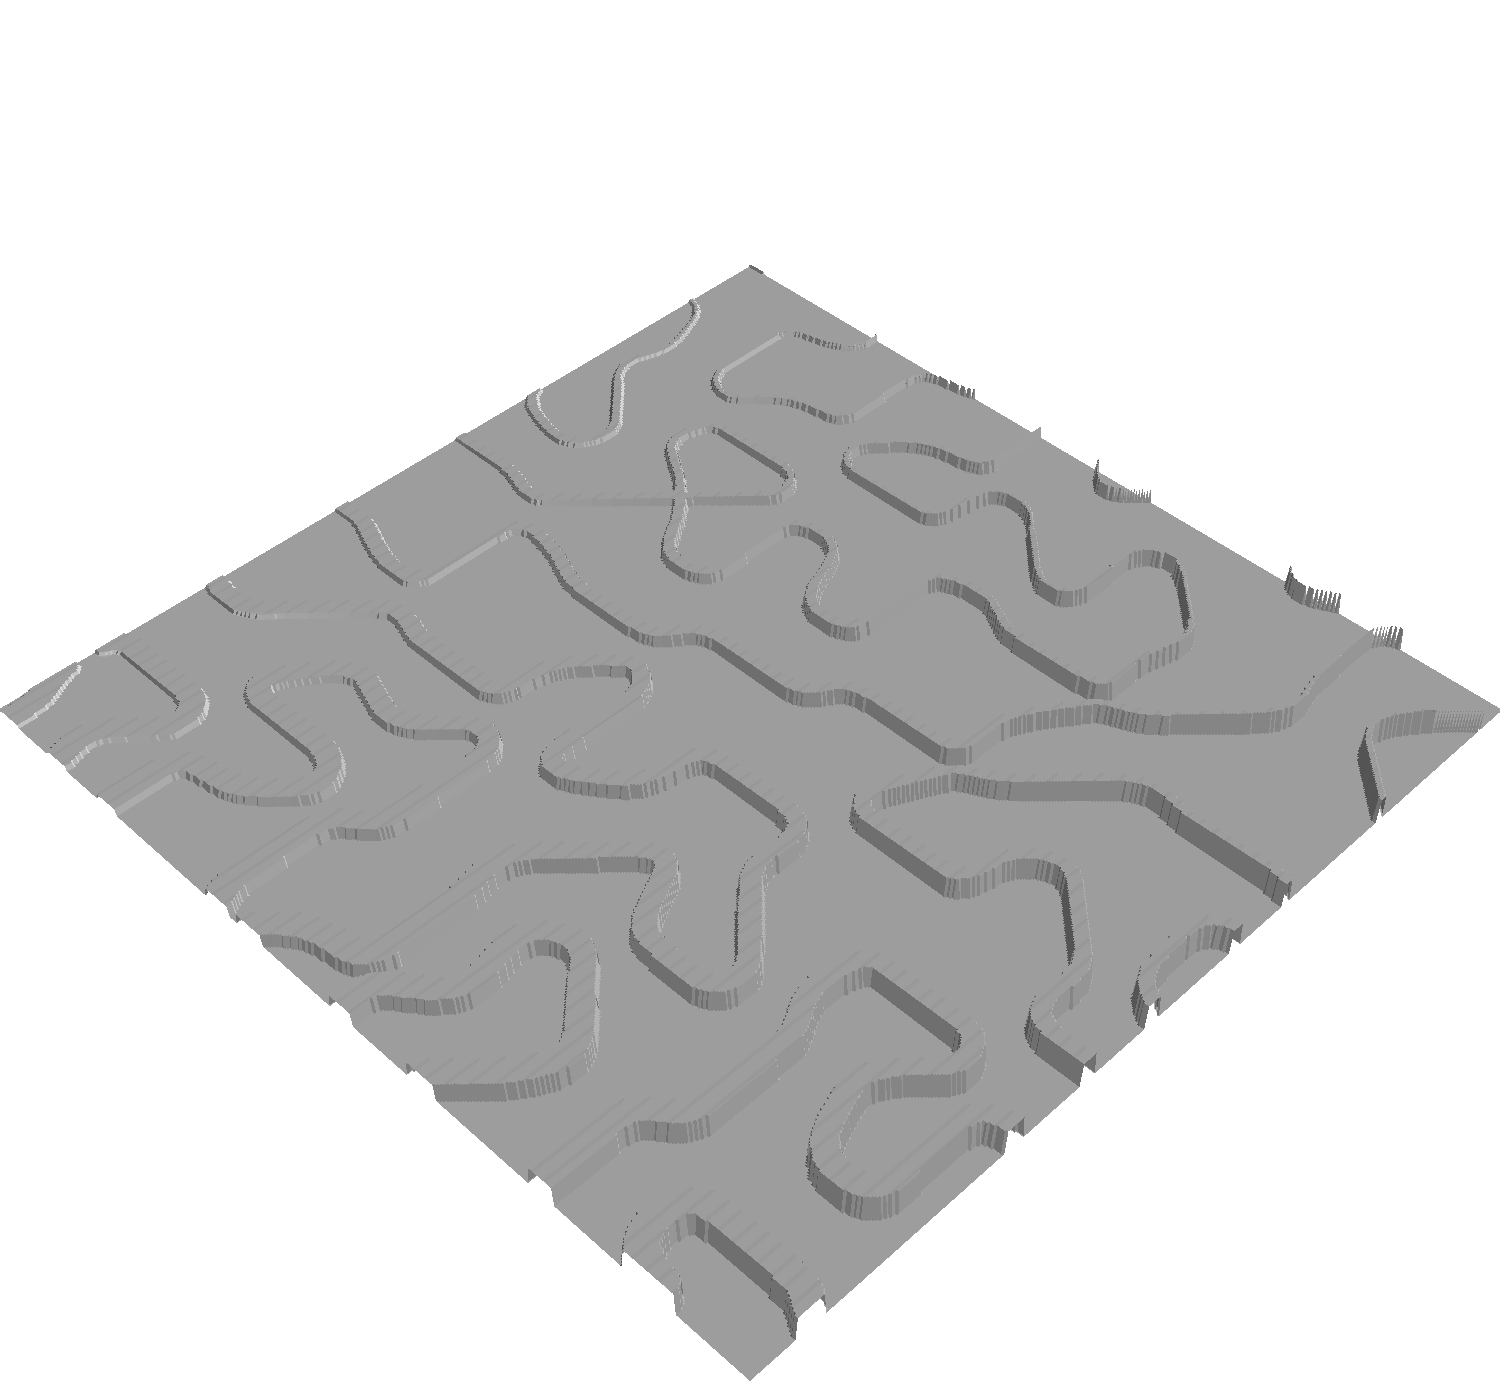
\includegraphics[width=\linewidth]{../img/hm3d/bars1.png}
        \caption{Walls.}
    \end{subfigure}
    \begin{subfigure}[b]{0.24\textwidth}
        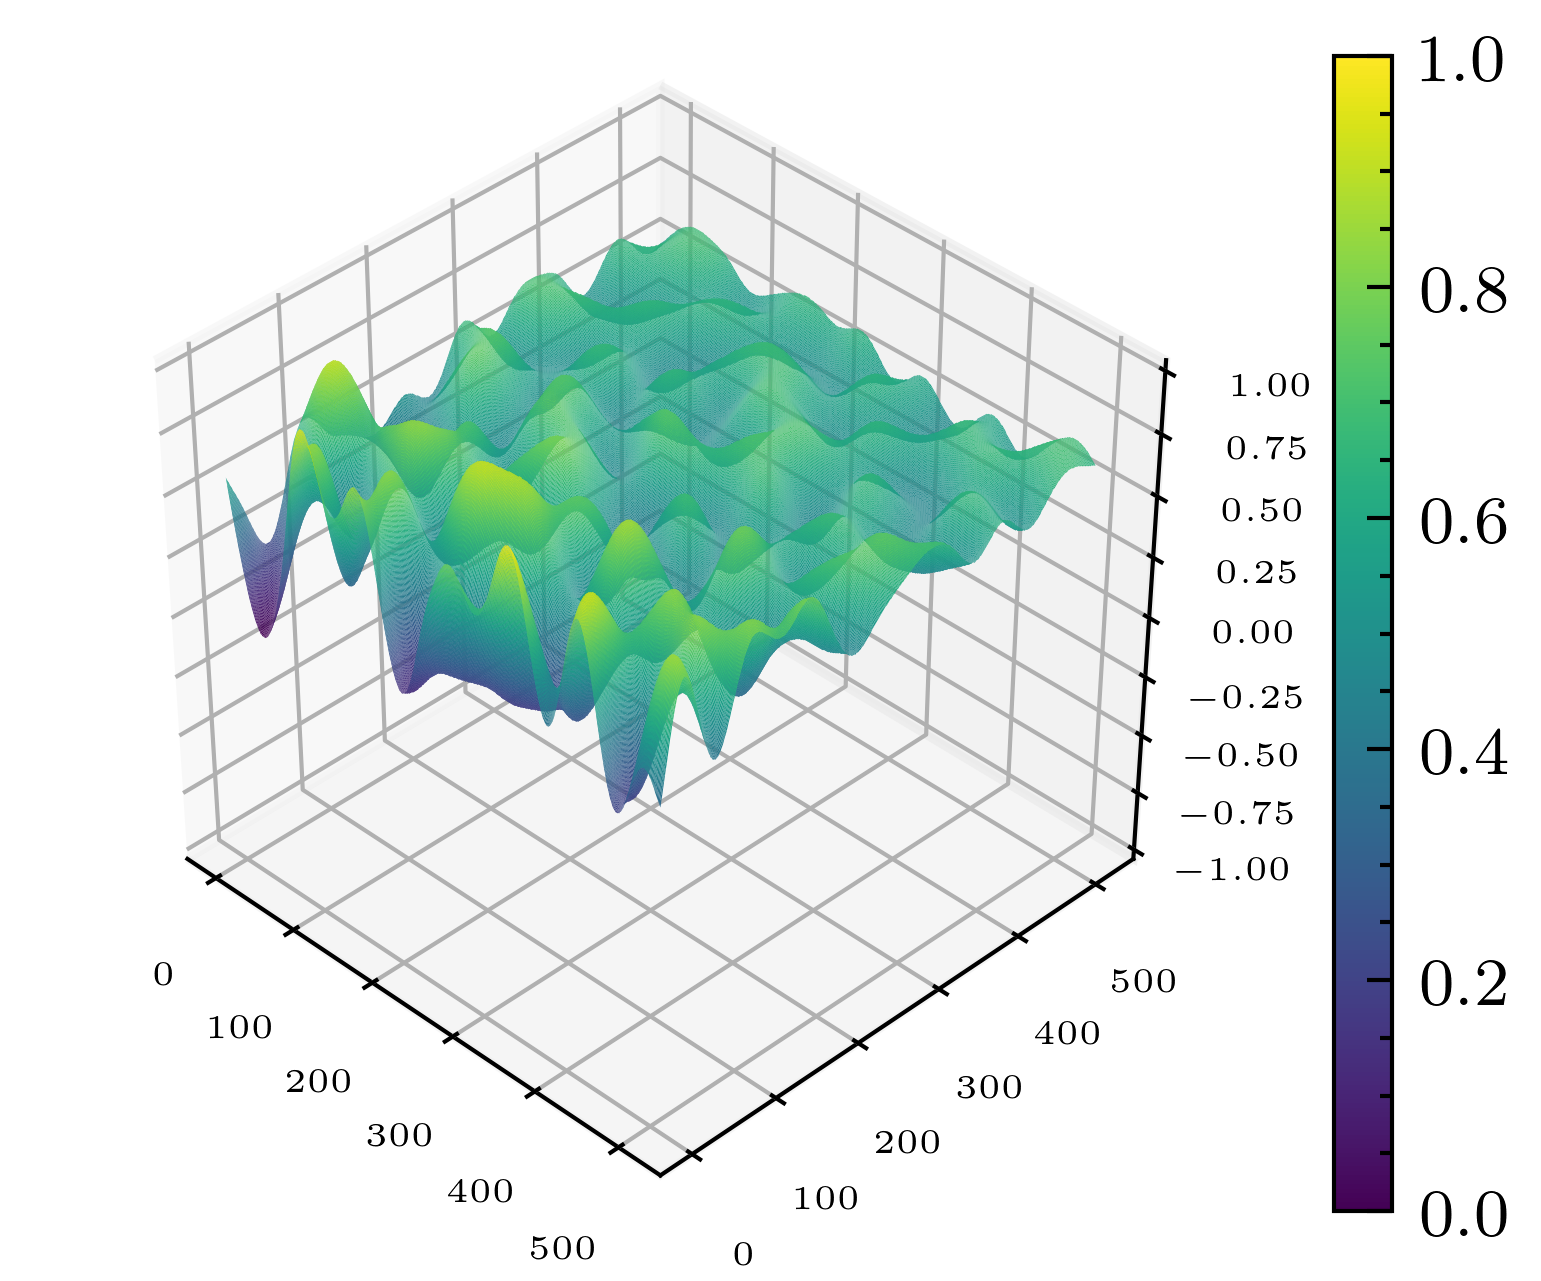
\includegraphics[width=\linewidth]{../img/hm3d/bumps2.png}
        \caption{Bumps.}
 \end{subfigure}  
    \begin{subfigure}[b]{0.24\textwidth}
        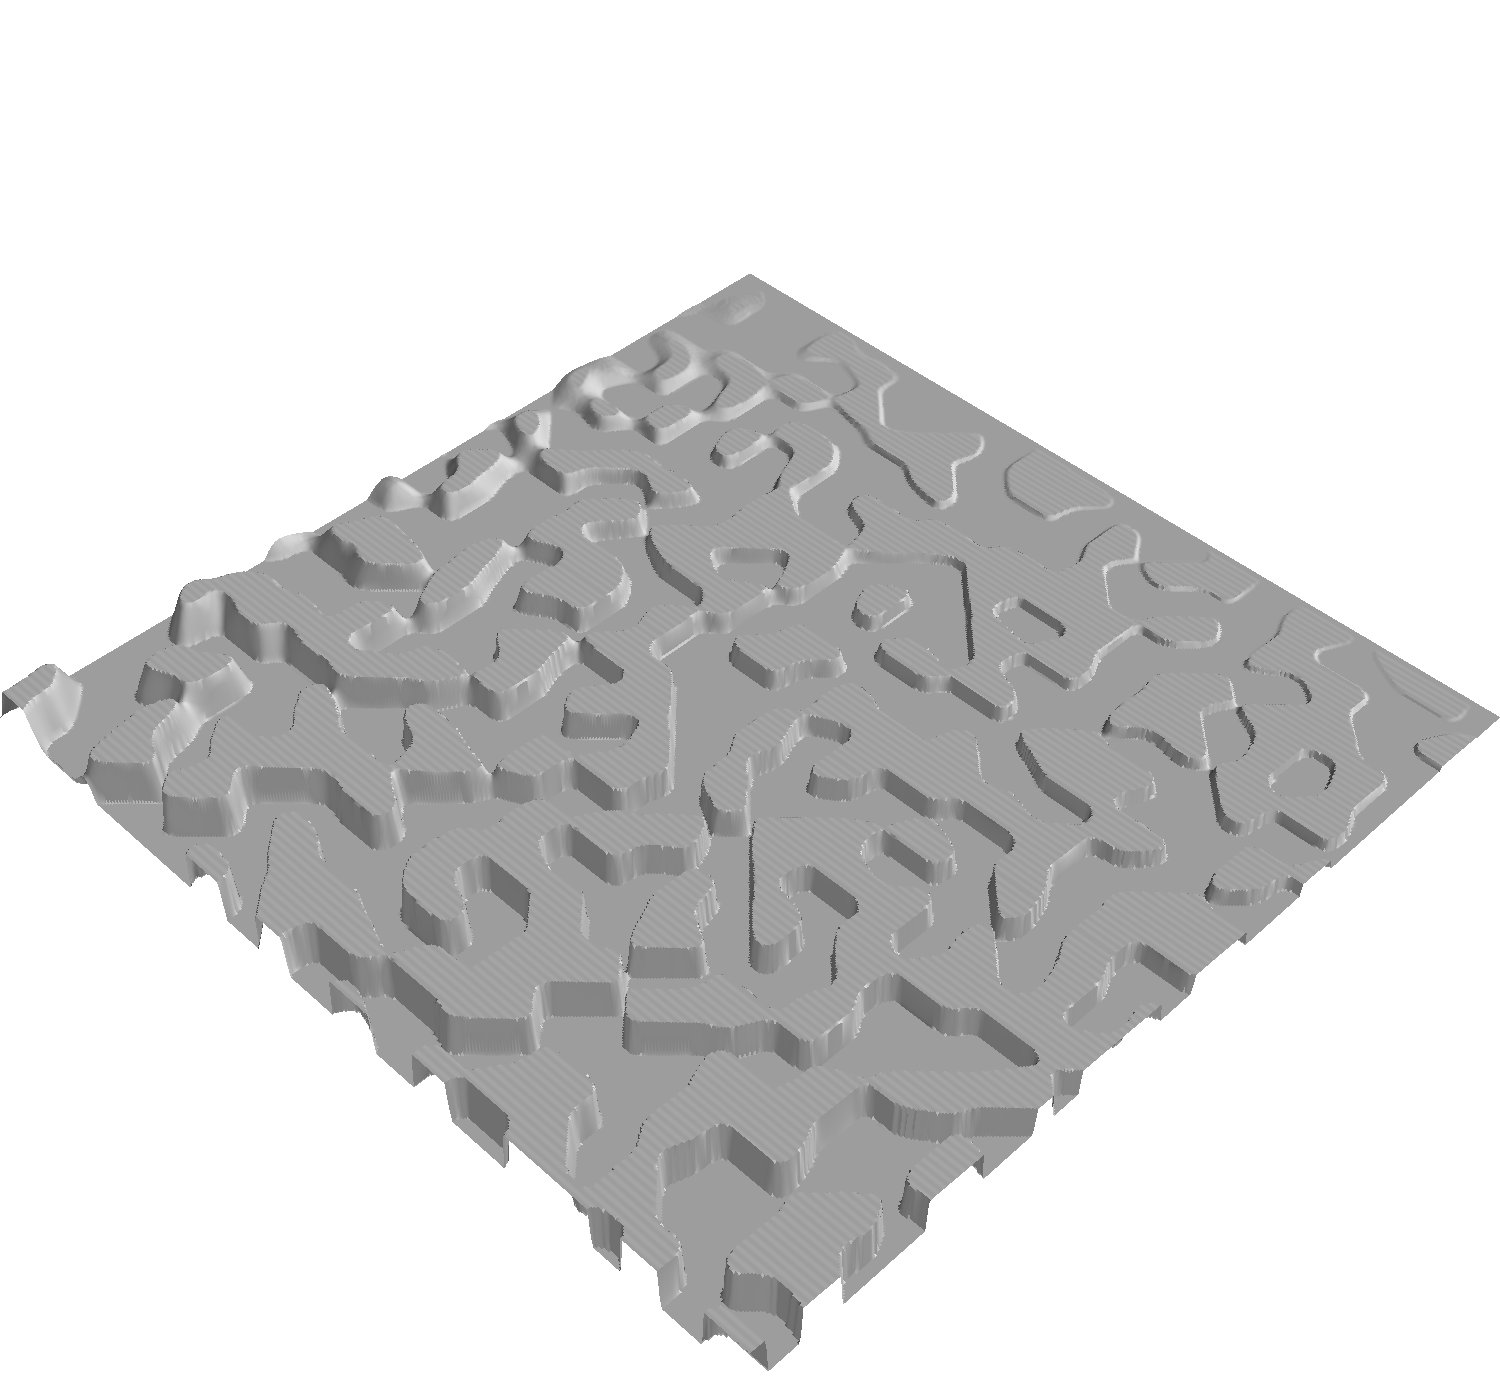
\includegraphics[width=\linewidth]{../img/hm3d/steps1.png}
        \caption{Steps.}
 \end{subfigure}  
    \begin{subfigure}[b]{0.24\textwidth}
        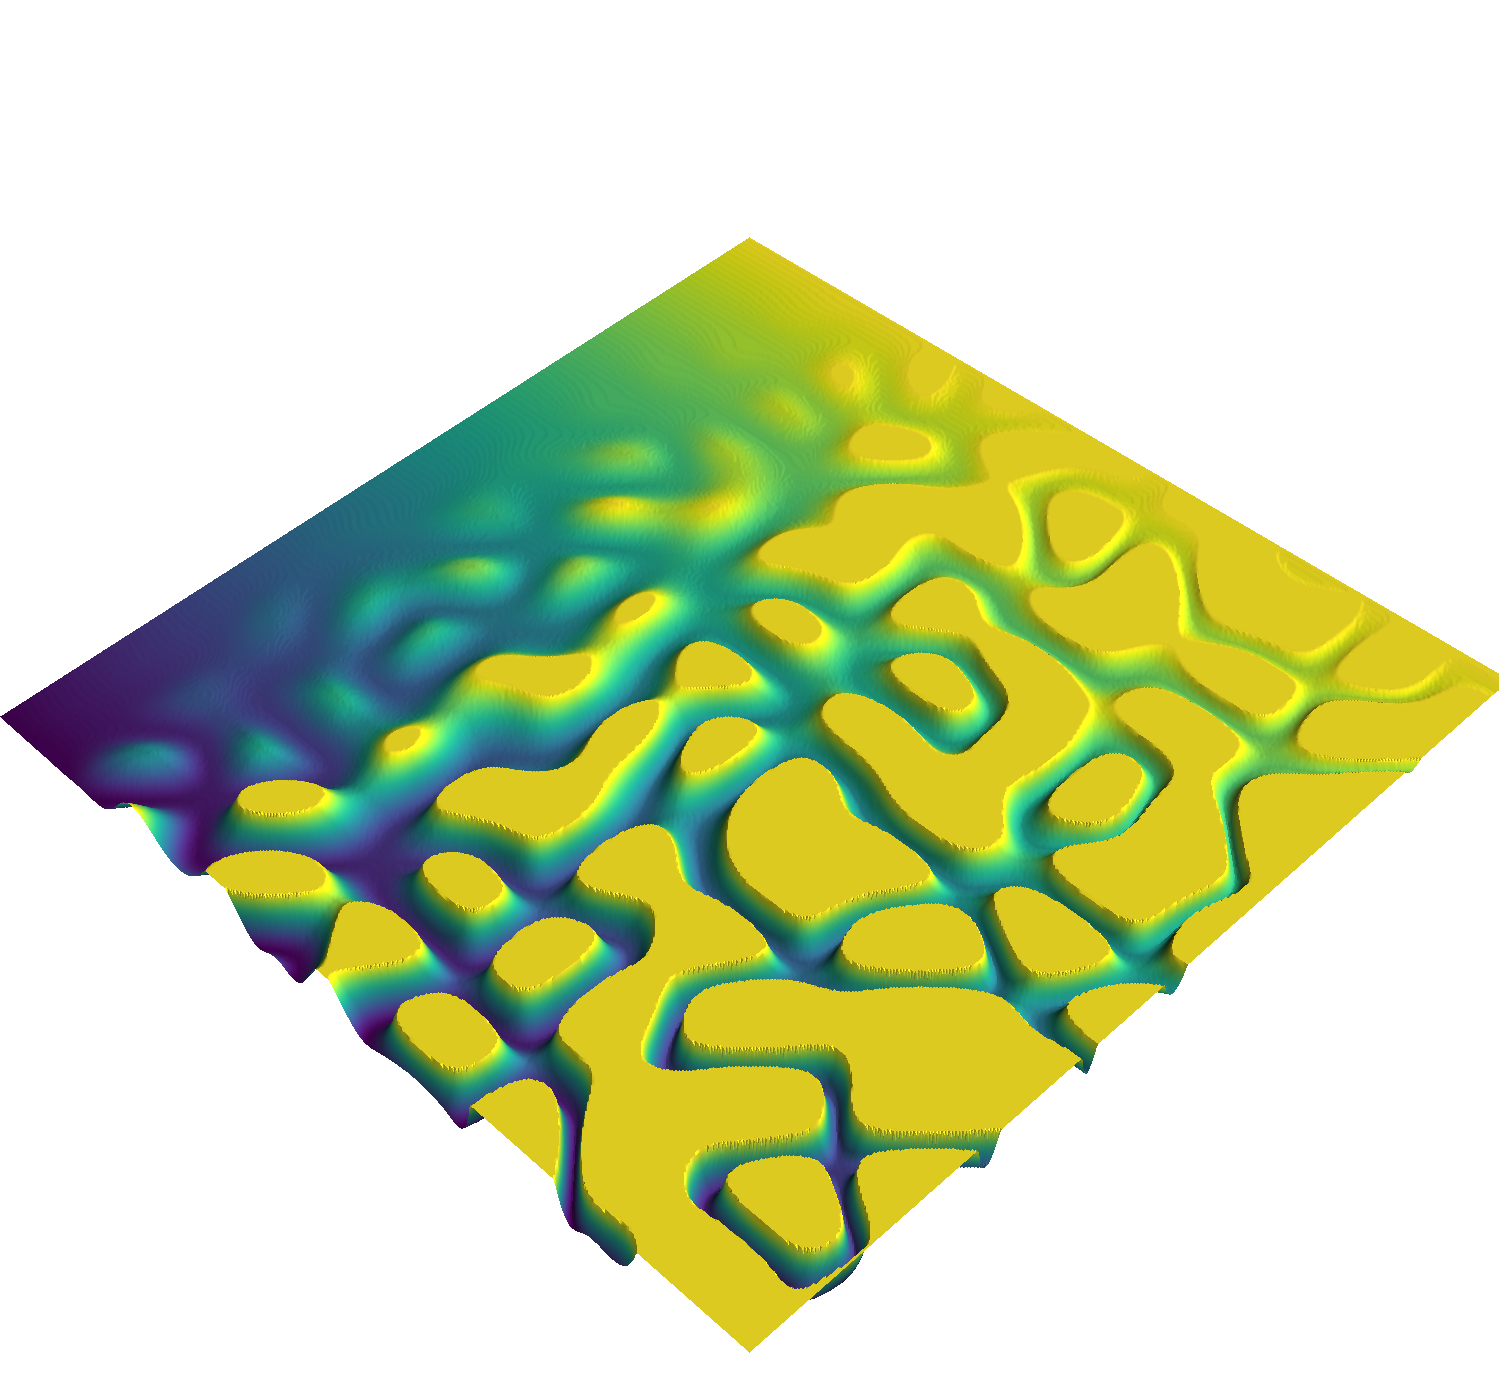
\includegraphics[width=\linewidth]{../img/hm3d/rails3.png}
        \caption{Rails.}
    \end{subfigure}  
\caption{Some artificially generated terrains, $10\times 10$m, with one specific feature each. }   
\end{figure}
To let the robot interacts with them, each map can be simply loaded into a simulator. To ensure a correct exploration of each terrain, it is better to randomly spawn the robot multiple times on the same map and let it walk for a fixed amount of time. The robot position is tracked and stored during simulation in order to extract a small portion of ground, patches, around each of its trajectory's position. In practice, the patches are cropped from the original image using a specific size based on the robot's footprint and its velocity. Each resulting image is labeled using a minimum advancement based on the robot's characteristic. We tested our framework on a legged crocodile-like robot called \emph{Krock}. Due to its four legs, the robot has very unique locomotion allowing it to overcome different obstacles making estimate traversability more challenging. Figure \ref{patch-extraction} helps to visualize the procedure.
\begin{figure}[H]
    \centering
    \begin{subfigure}[b]{0.66\textwidth}
    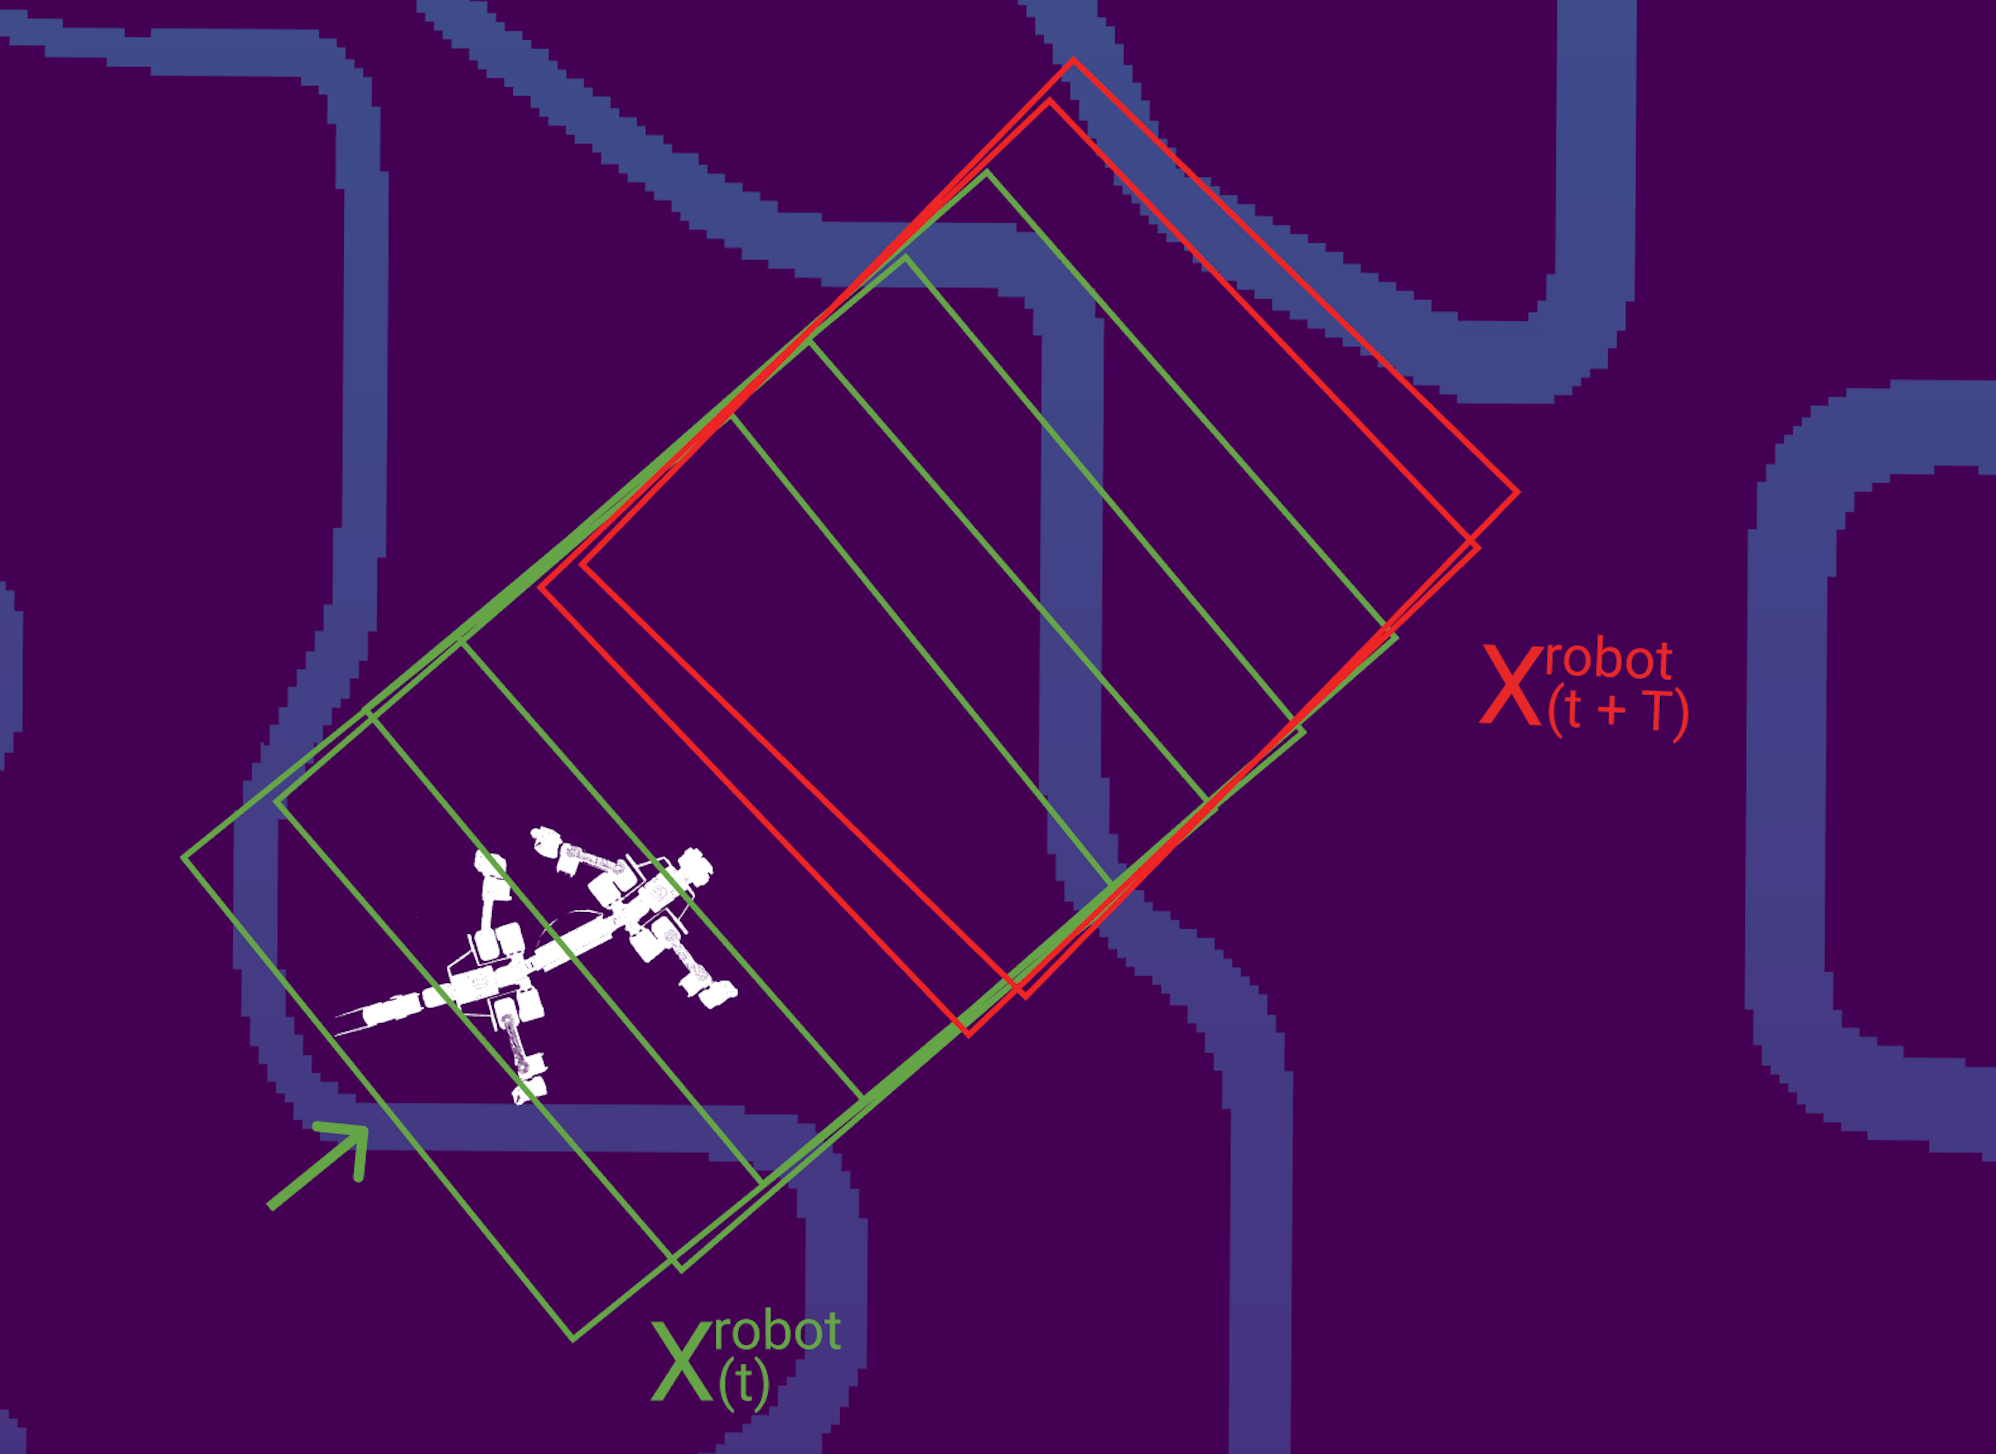
\includegraphics[width=\textwidth]{../img/krock-bars-correct-small.png}
    \caption{Robot's trajectory.}
\end{subfigure}
\begin{subfigure}[b]{1\textwidth}
    \begin{subfigure}[b]{0.19\textwidth}
    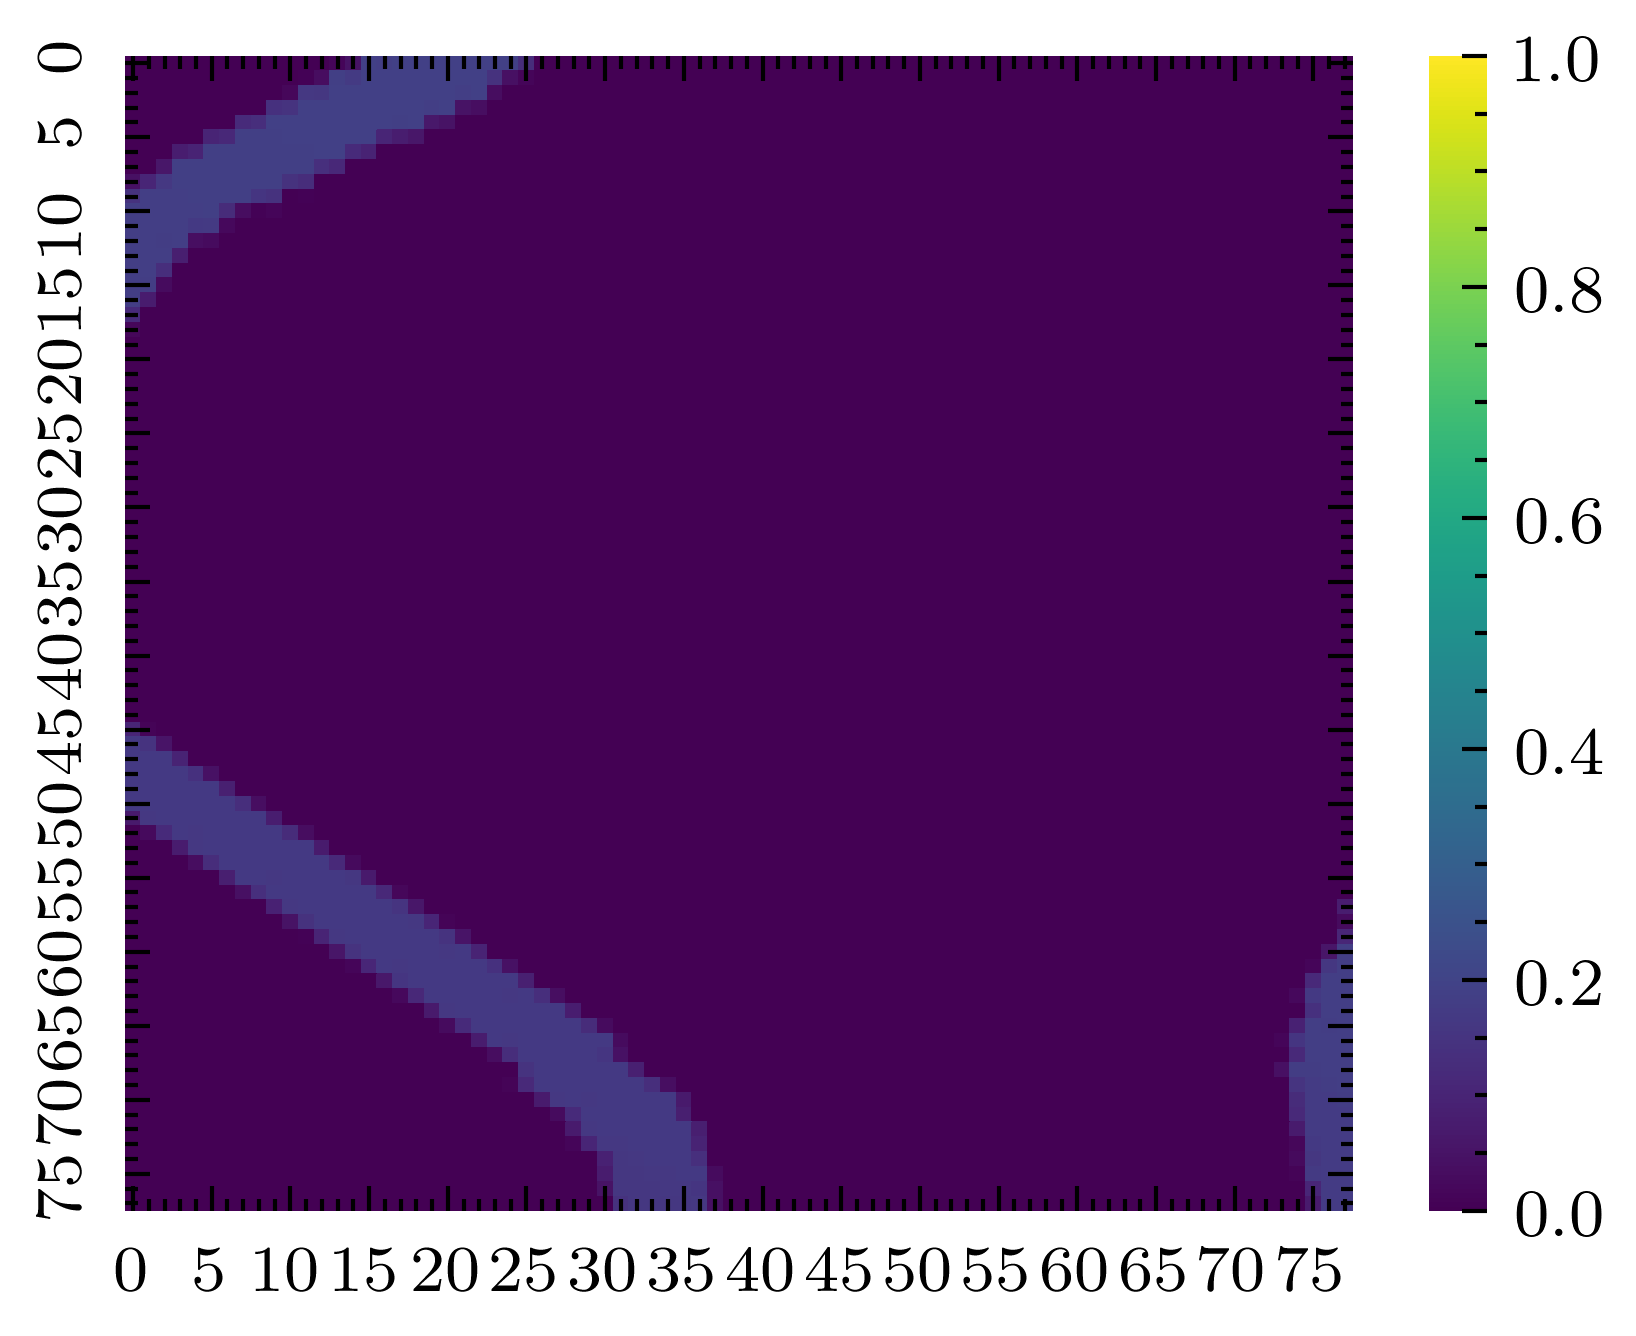
\includegraphics[width=\linewidth]{../img/bars1-example-patches/2d/0.png}
    \end{subfigure}
    \begin{subfigure}[b]{0.19\textwidth}
    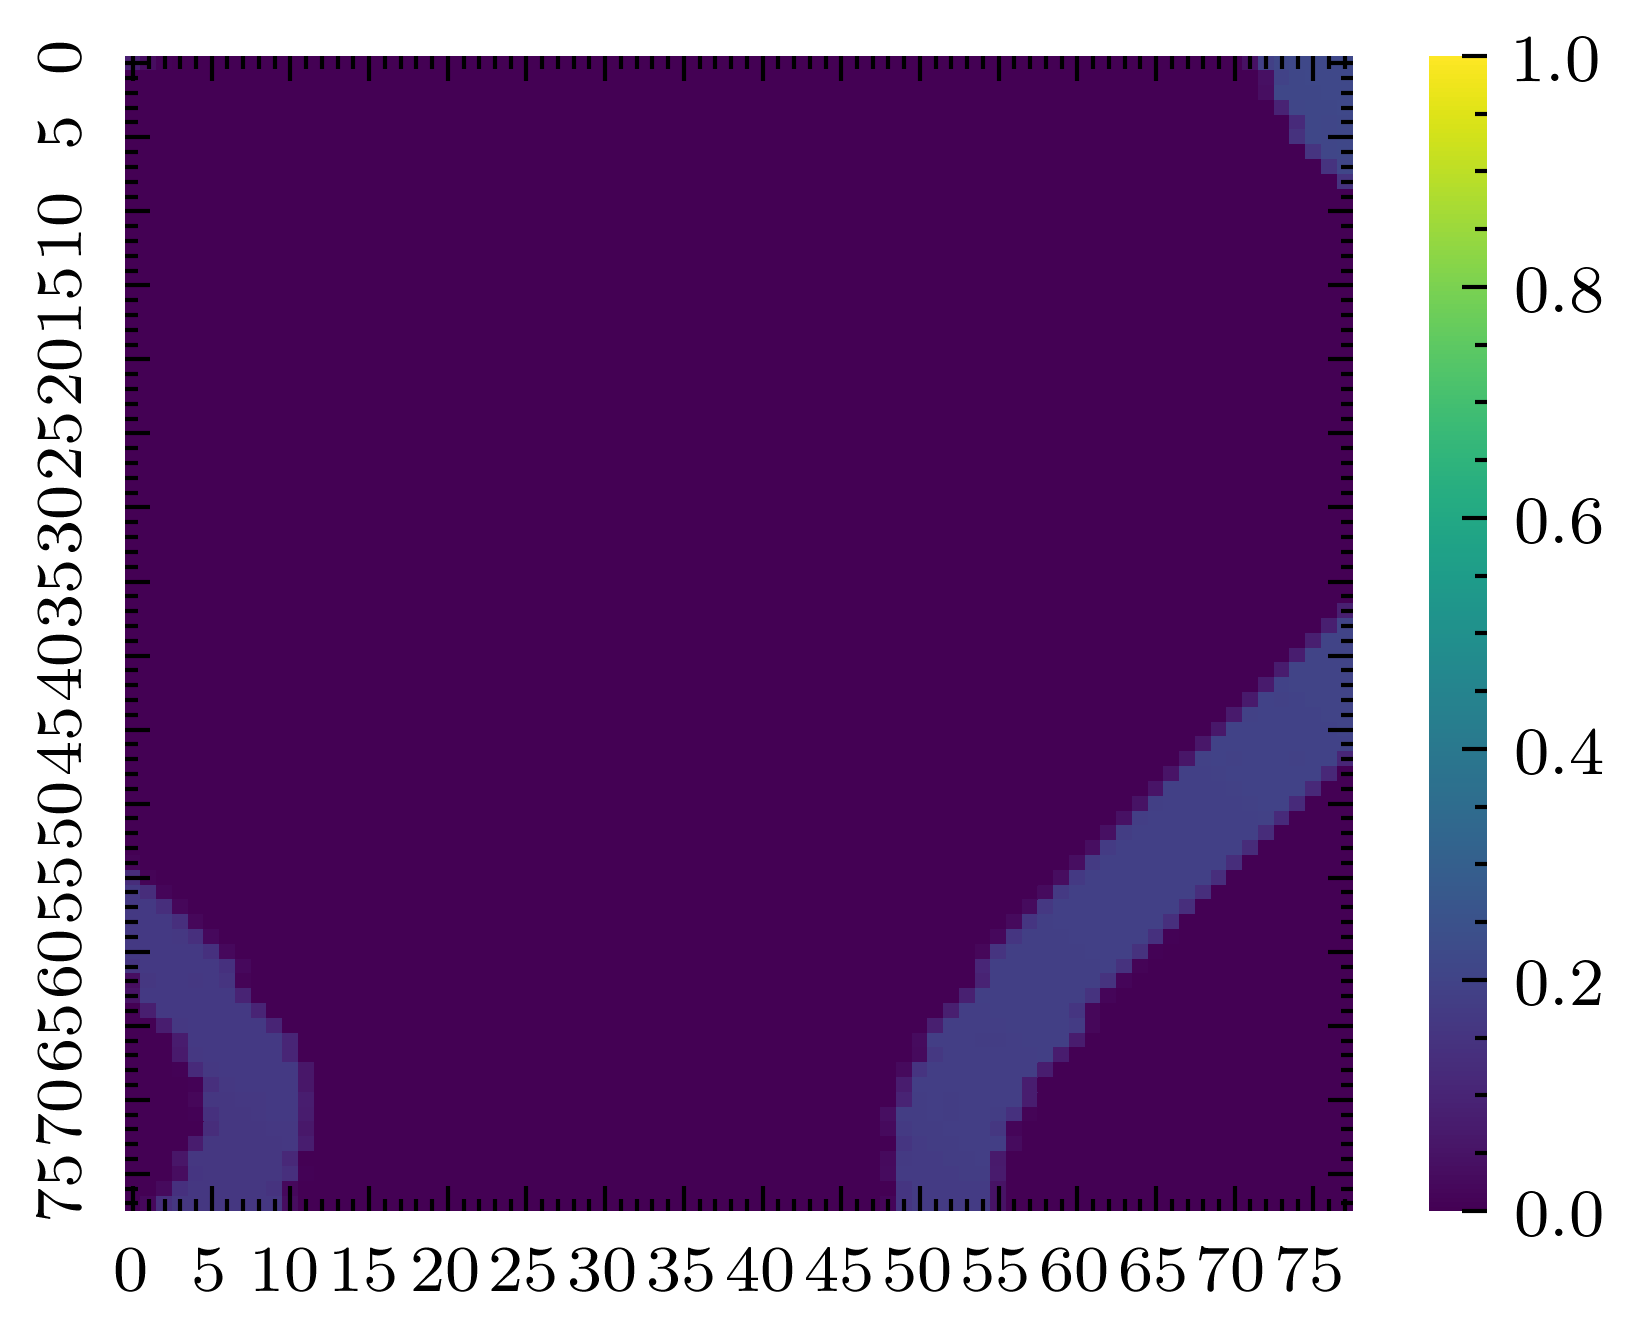
\includegraphics[width=\linewidth]{../img/bars1-example-patches/2d/2.png}    
    \end{subfigure}  
    \begin{subfigure}[b]{0.19\textwidth}
    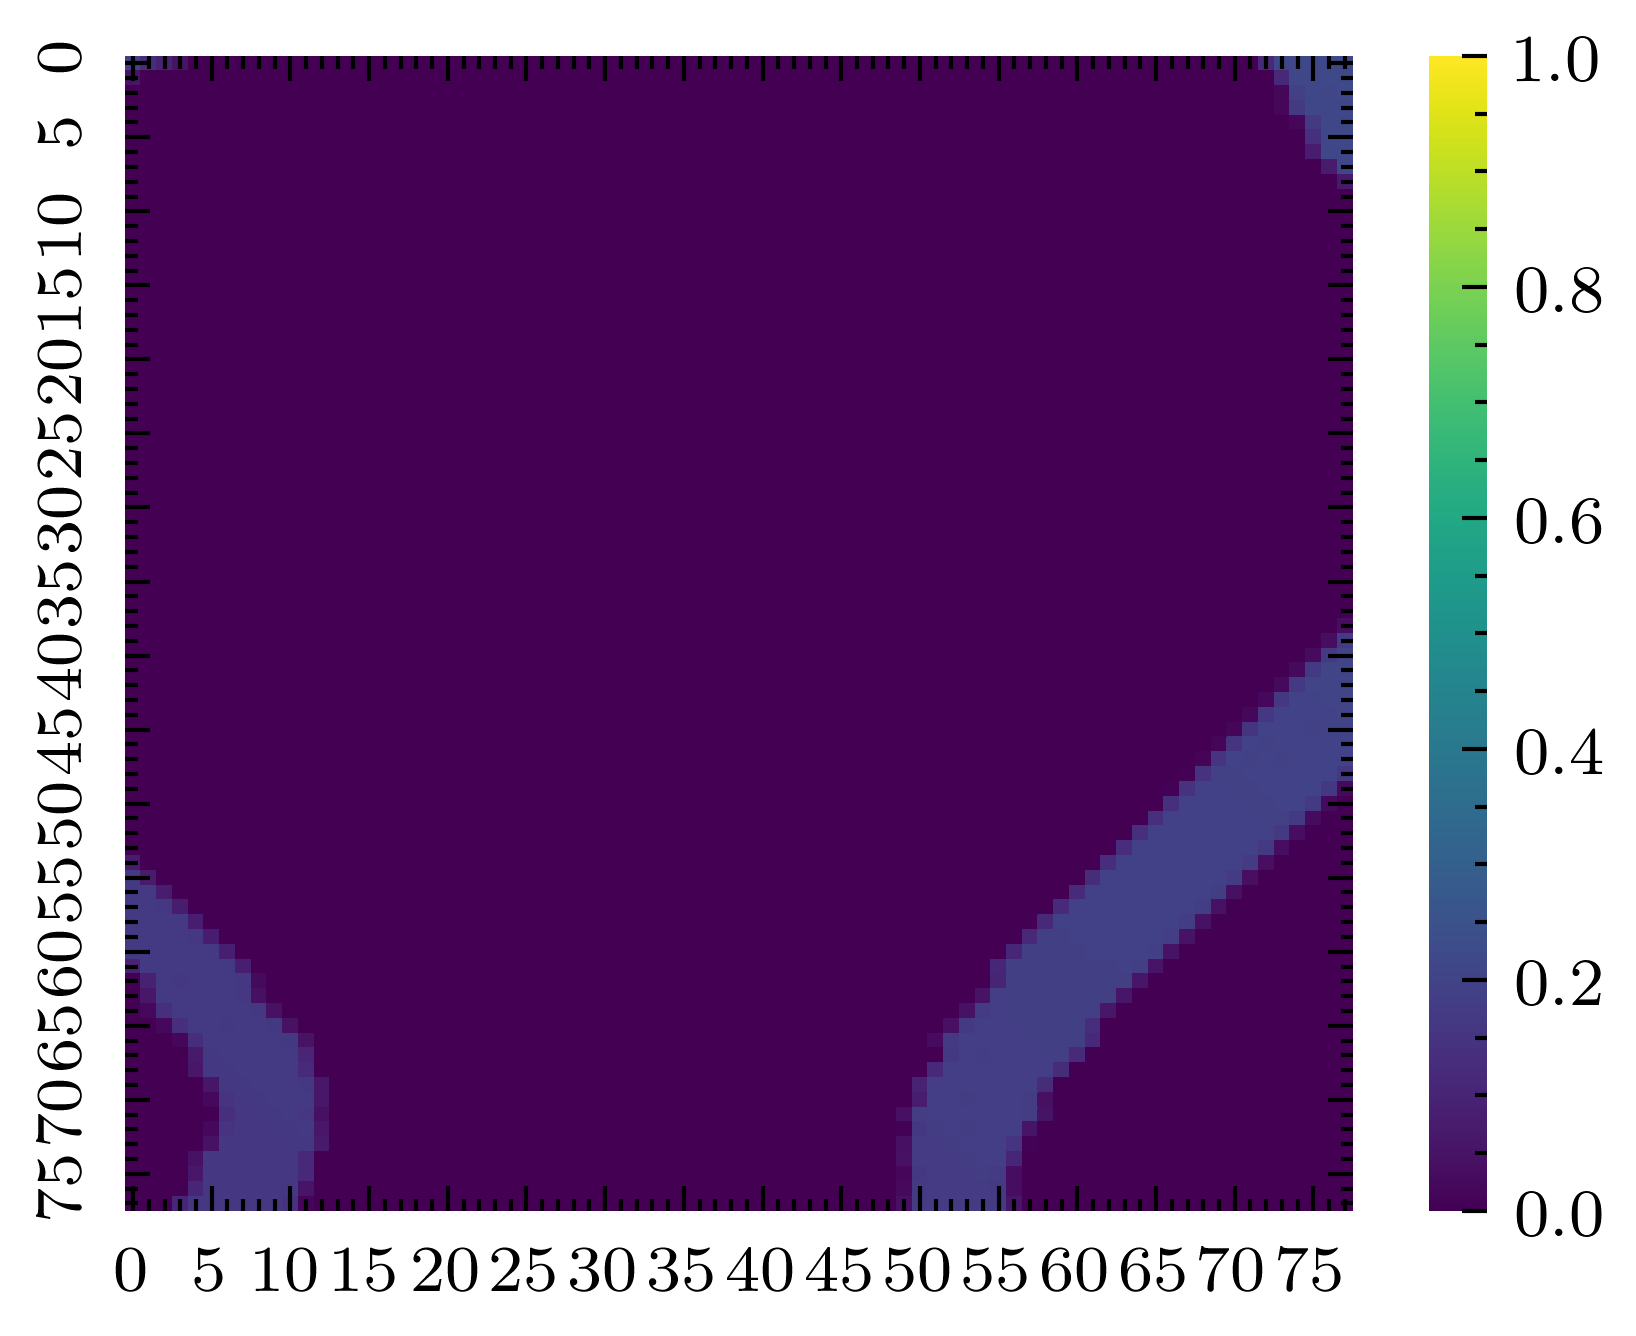
\includegraphics[width=\linewidth]{../img/bars1-example-patches/2d/4.png} 
    \end{subfigure}
    \begin{subfigure}[b]{0.19\textwidth}
    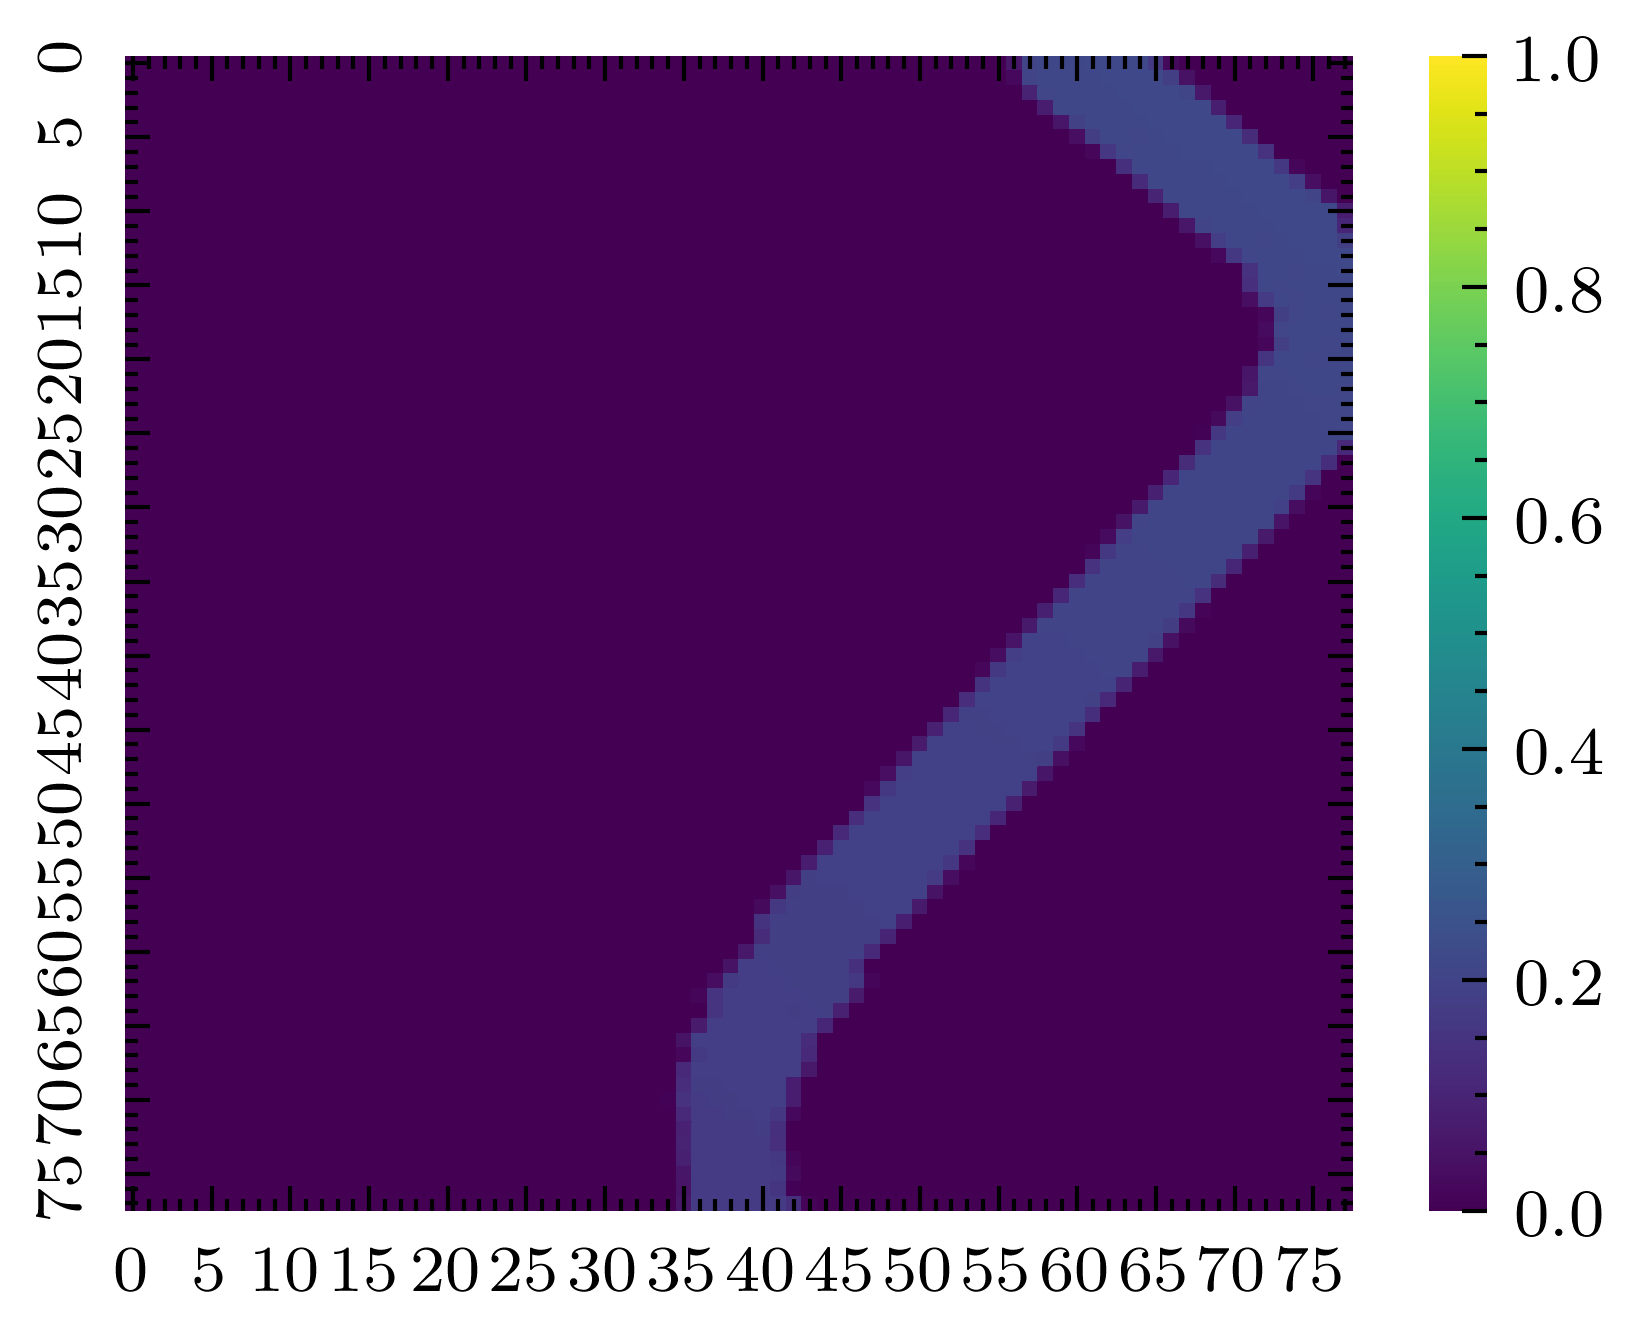
\includegraphics[width=\linewidth]{../img/bars1-example-patches/2d/7.png}    
    \end{subfigure}  
    \begin{subfigure}[b]{0.19\textwidth}
    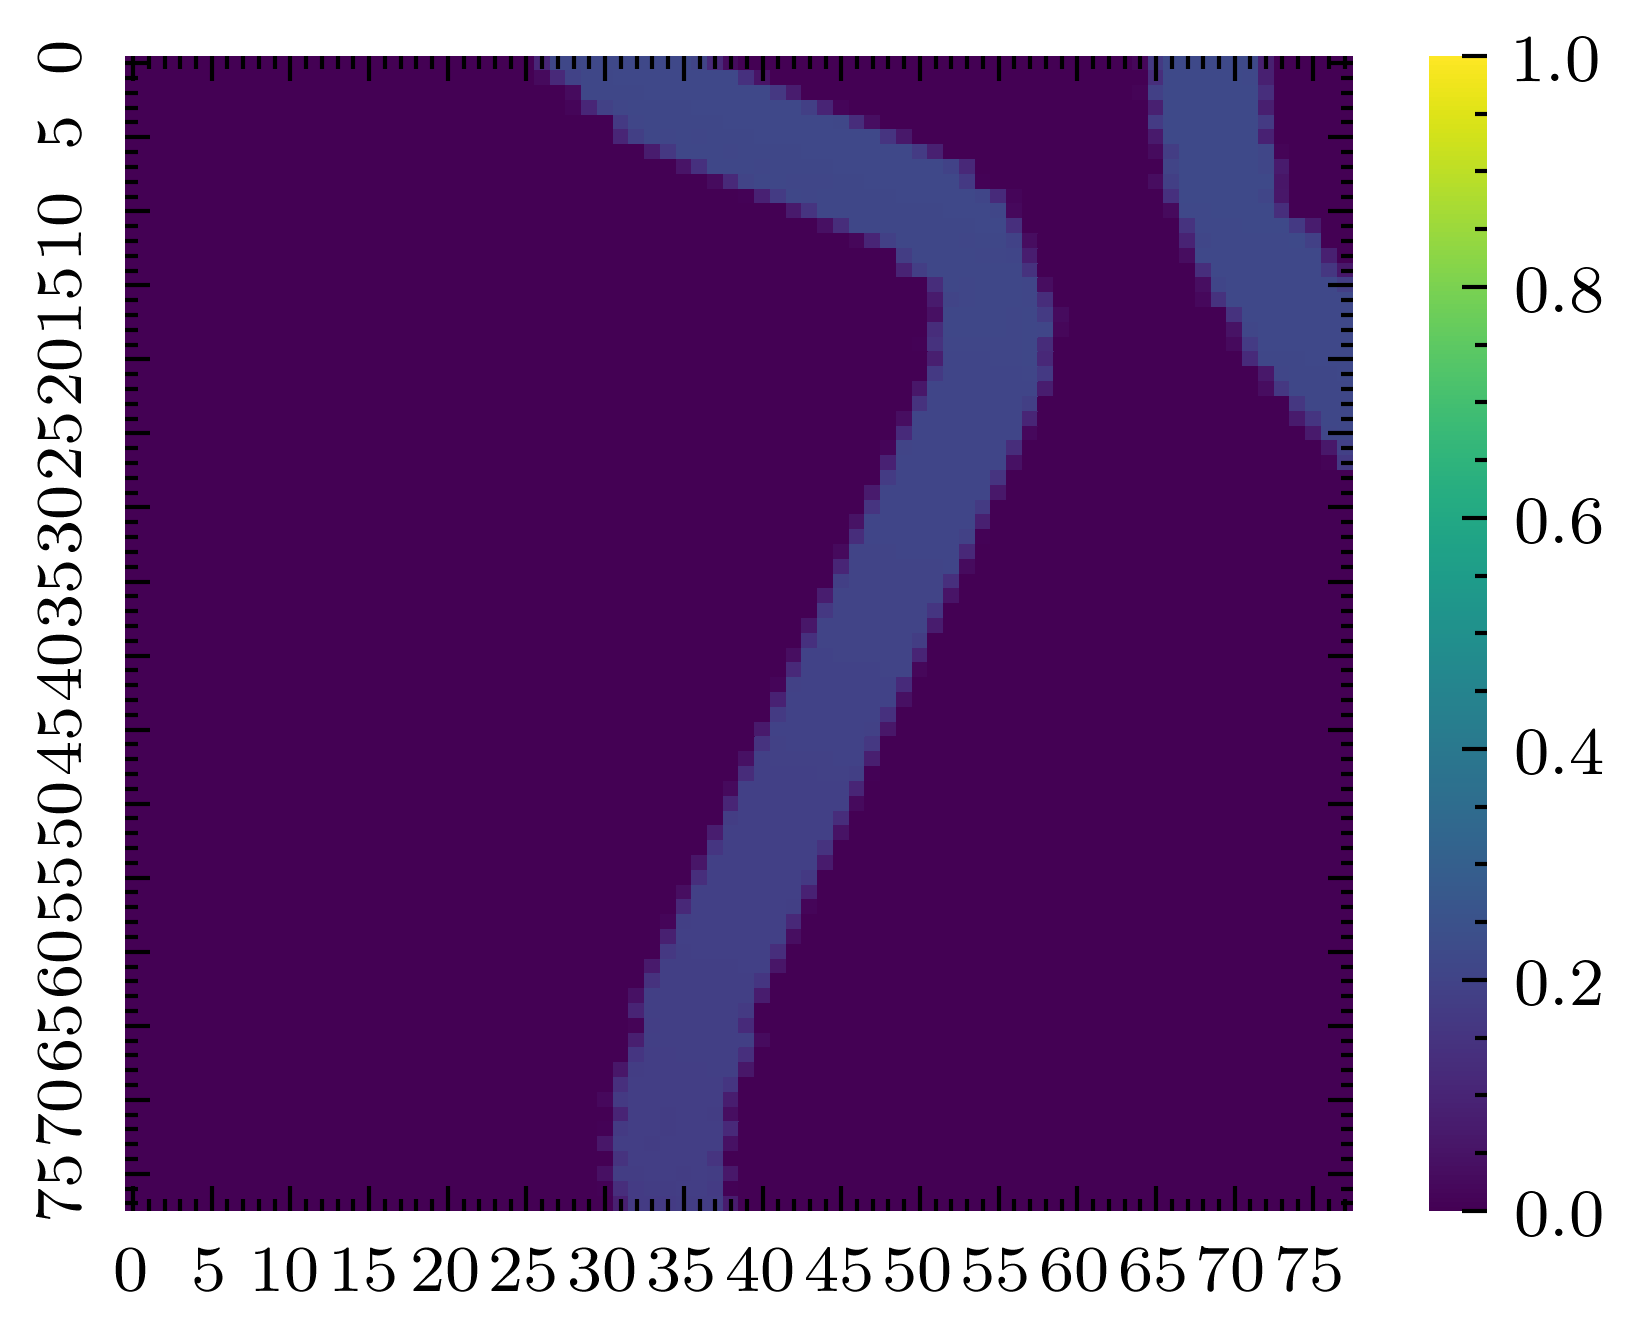
\includegraphics[width=\linewidth]{../img/bars1-example-patches/2d/14.png}    
    \end{subfigure}  
\caption{Cropped patches in 2D.}
\end{subfigure}  
\begin{subfigure}[b]{1\textwidth}
    \begin{subfigure}[b]{0.19\textwidth}
    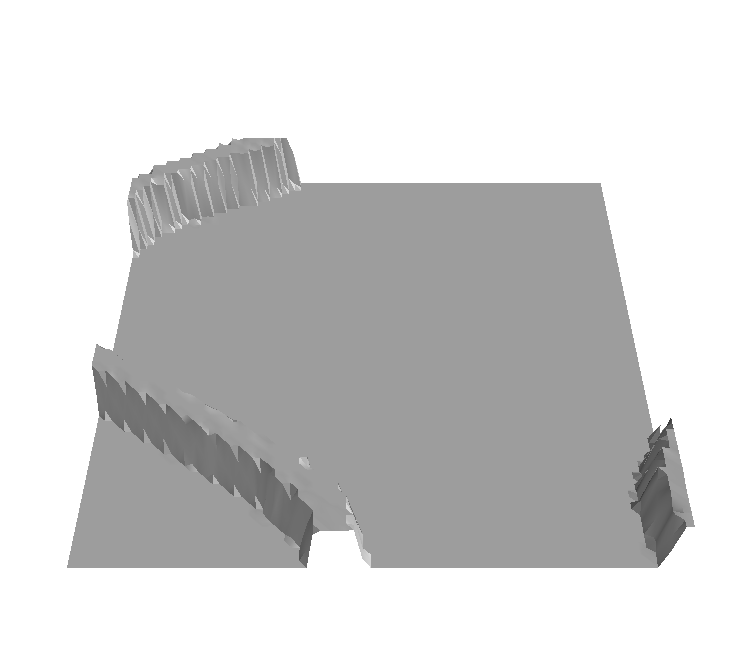
\includegraphics[width=\linewidth]{../img/bars1-example-patches/3d/0.png}
    \end{subfigure}
    \begin{subfigure}[b]{0.19\textwidth}
    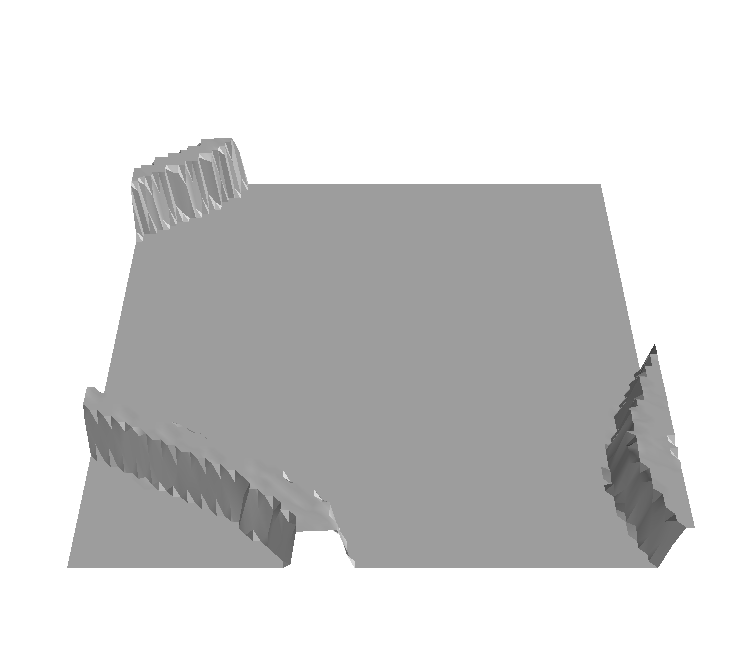
\includegraphics[width=\linewidth]{../img/bars1-example-patches/3d/2.png}    
    \end{subfigure}  
    \begin{subfigure}[b]{0.19\textwidth}
    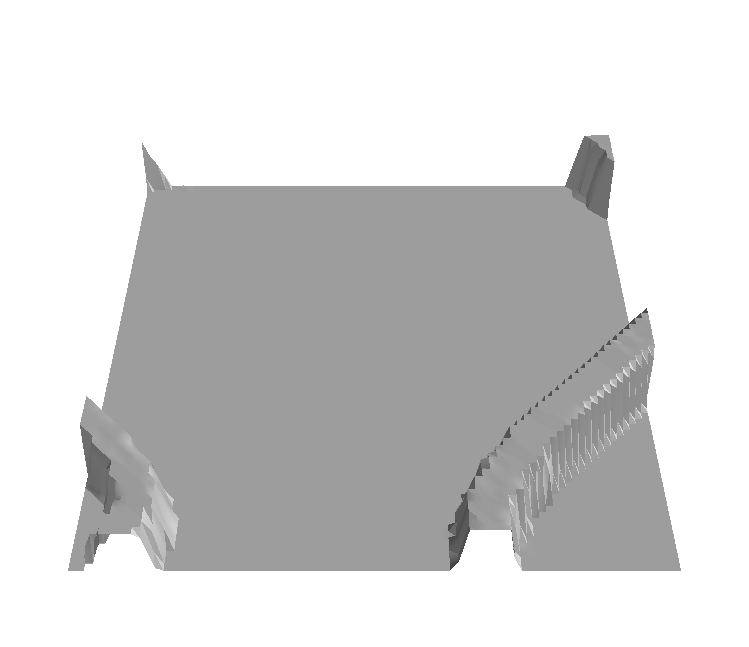
\includegraphics[width=\linewidth]{../img/bars1-example-patches/3d/4.png} 
    \end{subfigure}
    \begin{subfigure}[b]{0.19\textwidth}
    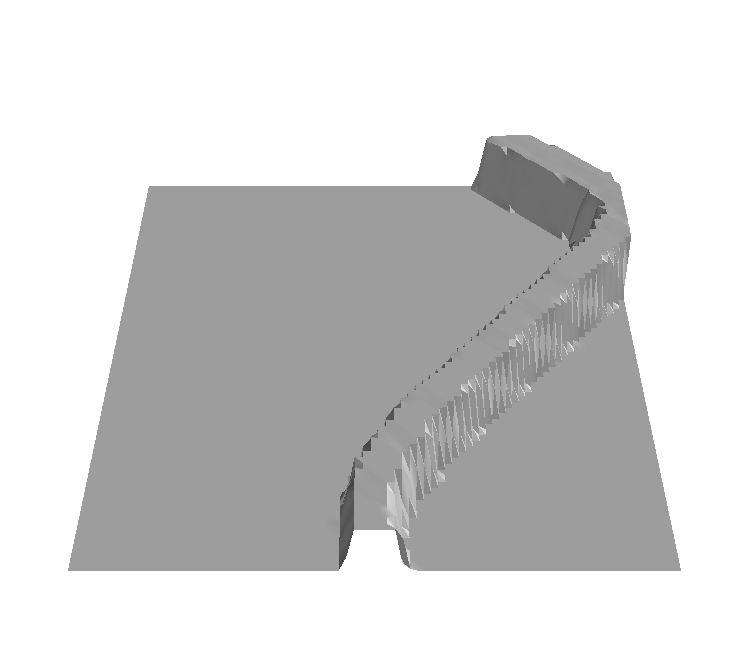
\includegraphics[width=\linewidth]{../img/bars1-example-patches/3d/7.png}    
    \end{subfigure}  
    \begin{subfigure}[b]{0.19\textwidth}
    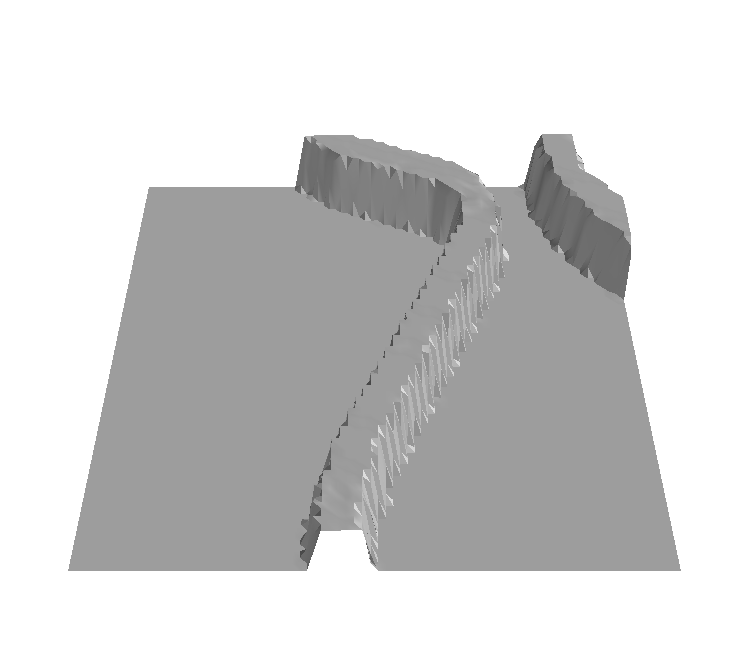
\includegraphics[width=\linewidth]{../img/bars1-example-patches/3d/14.png}    
    \end{subfigure}  
\caption{Cropped patches in 3D.}
\label{fig : patch-extraction}
\end{subfigure}
\caption{Example of a robot trajectory (a) extracted during training on a map with different walls. Robot's initial position is shown by its white silhouette. Patches borders are labeled with greed if traversable and red if not and showed as 2D (b) and 3D(c) rendered images. The robot traverses the patches from left to right.}
\end{figure}

This dataset is fed to a deep convolutional neural network. The network directly learns to extract features from raw data, in our case images, without needing to preprocess the inputs. We utilized a model three times lighter than the original one with comparable performance. We evaluated all tested architecture using real-world terrains, mostly obtained with flying droned and ground mapping software. 
We also investigate the model's learning by first visualizing the inputs that confuse the model. We adopted a technique that allows highlighting the regions in the input images that contribute the most to the prediction, in this way we can understand which part of the terrain was responsible for the wrong prediction. Lastly, we tested the model's robustness by creating different patches with different characteristics and compare the prediction to the ground truth from the simulator. We shown that the model was able to match the simulator's outputs in most scenarios but most important, we understandood the network's limitations.

To summarize our contributions to literature are the implementation of a framework to learn traversability entirely through simulation data that can be employed with any mobile robot, a new small neural network architecture able to reach high accuracy, different real-world evaluations, and a model interpretability case study to understand the strengths and limitations of the trained model. 

\end{document}
